\documentclass[tikz]{standalone}

\usetikzlibrary{calc,positioning,shapes,positioning,intersections,quotes,decorations.markings}
\usepackage{amsfonts,amsmath,amsthm,amssymb,mathtools,stmaryrd,mathrsfs}

\begin{document}
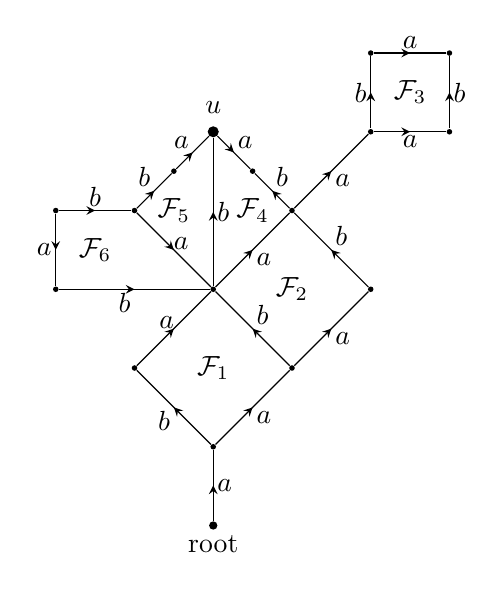
\begin{tikzpicture}[>=stealth,decoration={
				markings,
				mark=at position 0.5 with {\arrow{>}}}
	]

	\node[circle,fill=black,inner sep=0pt,minimum size=3pt] (root) at (0,0){} node[below]{root};
	\node[circle,fill=black,inner sep=0pt,minimum size=2pt] (n1) at (0,1) {};
	\node[circle,fill=black,inner sep=0pt,minimum size=2pt] (n2) at (1,2) {};
	\node[circle,fill=black,inner sep=0pt,minimum size=2pt] (n3) at (0,3) {};
	\node[circle,fill=black,inner sep=0pt,minimum size=2pt] (n4) at (-1,2) {};

	\draw[postaction={decorate}] (root) --node[right=-2pt]{$a$} (n1);
	\draw[postaction={decorate}] (n1) --node[below right=-3pt]{$a$} (n2);
	\draw[postaction={decorate}] (n2) --node[above right=-3pt]{$b$} (n3);
	\draw[postaction={decorate}] (n4) --node[above left=-5pt]{$a$} (n3);
	\draw[postaction={decorate}] (n1) --node[below left=-3pt]{$b$} (n4);

	\node[circle,fill=black,inner sep=0pt,minimum size=2pt] (n5) at (2,3) {};
	\node[circle,fill=black,inner sep=0pt,minimum size=2pt] (n6) at (1,4) {};

	\draw[postaction={decorate}] (n2) --node[below right=-3pt]{$a$} (n5);
	\draw[postaction={decorate}] (n5) --node[above right=-3pt]{$b$} (n6);
	\draw[postaction={decorate}] (n3) --node[below right=-3pt]{$a$} (n6);

	\node[circle,fill=black,inner sep=0pt,minimum size=2pt] (n7) at (0.5,4.5) {};
	\node[circle,fill=black,inner sep=0pt,minimum size=4pt] (n8) at (0,5) {};

  % label
  \node[above=0.1em of n8] {$u$};

	\draw[postaction={decorate}] (n3) --node[right=-2pt]{$b$} (n8);
	\draw[postaction={decorate}] (n8) --node[above right=-3pt]{$a$} (n7);
	\draw[postaction={decorate}] (n6) --node[above right=-3pt]{$b$} (n7);

	\node[circle,fill=black,inner sep=0pt,minimum size=2pt] (n9) at (-0.5,4.5) {};
	\node[circle,fill=black,inner sep=0pt,minimum size=2pt] (n10) at (-1,4) {};

	\draw[postaction={decorate}] (n10) --node[above right=-5pt]{$a$} (n3);
	\draw[postaction={decorate}] (n10) --node[above left=-3pt]{$b$} (n9);
	\draw[postaction={decorate}] (n9) --node[above left=-3pt]{$a$} (n8);

	\node[circle,fill=black,inner sep=0pt,minimum size=2pt] (n11) at (-2,4) {};
	\node[circle,fill=black,inner sep=0pt,minimum size=2pt] (n12) at (-2,3) {};

	\draw[postaction={decorate}] (n12) --node[below left=-3pt]{$b$} (n3);
	\draw[postaction={decorate}] (n11) --node[left=-2pt]{$a$} (n12);
	\draw[postaction={decorate}] (n11) --node[above=-2pt]{$b$} (n10);

	\node[circle,fill=black,inner sep=0pt,minimum size=2pt] (n13) at (2,5) {};
	\node[circle,fill=black,inner sep=0pt,minimum size=2pt] (n14) at (3,5) {};
	\node[circle,fill=black,inner sep=0pt,minimum size=2pt] (n15) at (3,6) {};
	\node[circle,fill=black,inner sep=0pt,minimum size=2pt] (n16) at (2,6) {};

	\draw[postaction={decorate}] (n6) --node[below right=-3pt]{$a$} (n13);
	\draw[postaction={decorate}] (n13) --node[below=-2pt]{$a$} (n14);
	\draw[postaction={decorate}] (n14) --node[right=-2pt]{$b$} (n15);
	\draw[postaction={decorate}] (n13) --node[left=-2pt]{$b$} (n16);
	\draw[postaction={decorate}] (n16) --node[above=-2pt]{$a$} (n15);

  \node (f1) at (0,2) {$\mathcal F_1$};
  \node (f2) at (1,3) {$\mathcal F_2$};
  \node (f3) at (2.5,5.5) {$\mathcal F_3$};
  \node (f4) at (0.5,4) {$\mathcal F_4$};
  \node (f5) at (-0.5,4) {$\mathcal F_5$};
  \node (f6) at (-1.5,3.5) {$\mathcal F_6$};


\end{tikzpicture}
\end{document}
